\documentclass[11pt, a4paper]{article}
\usepackage[margin=2cm]{geometry}
\usepackage{booktabs}
\usepackage{multirow}
\usepackage{colortbl}
\usepackage{array}
\usepackage{siunitx}
\usepackage{threeparttable}
\usepackage{xcolor}
\usepackage{tikz}
\usetikzlibrary{positioning}
\usepackage{pgfplots}
\pgfplotsset{compat=1.18}
\usepgfplotslibrary{fillbetween}
\usepackage{graphicx}
\usepackage{subcaption}
\usepackage{enumitem}
\usepackage{fontspec}
\usepackage{hyperref}
\usepackage{amssymb}
\usepackage{amsmath}

%% ============================================================
%% PRIMARY PALETTE — Palette 4: Lavender Haze & Lime
%% ============================================================
\definecolor{Primary}{RGB}{166, 148, 232}      % Lavender — our model
\definecolor{PrimaryDark}{RGB}{90, 72, 160}    % Dark lavender — borders
\definecolor{Secondary}{RGB}{171, 204, 110}    % Lime — baseline 1
\definecolor{SecondaryDark}{RGB}{95, 130, 40}  % Dark lime — borders
\definecolor{Tertiary}{RGB}{241, 184, 144}     % Peach — baseline 2
\definecolor{TertiaryDark}{RGB}{180, 110, 60}  % Dark peach — borders
\definecolor{Neutral}{RGB}{102, 112, 130}      % Steel gray
\definecolor{PaperBg}{RGB}{249, 247, 252}      % Lavender paper
\definecolor{Ink}{RGB}{45, 42, 60}             % Dark plum ink
\definecolor{TableSep}{RGB}{220, 218, 240}     % Lavender table separator

%% Legacy aliases (for archive section)
\definecolor{LavenderBg}{RGB}{220, 226, 250}
\definecolor{SoftGreen}{RGB}{163, 213, 117}
\definecolor{DarkGreen}{RGB}{55, 100, 16}
\definecolor{Coral}{RGB}{232, 131, 107}
\definecolor{SteelBlue}{RGB}{107, 142, 196}

%% ============================================================
%% TOP-ONLY ROUNDED CORNERS FOR BARS
%% ============================================================
%% SHARED PGFPLOTS STYLE
%% ============================================================
\pgfplotsset{
    thesis bar/.style={
        ybar=3pt,
        width=0.85\textwidth,
        height=6cm,
        ylabel style={font=\small},
        tick label style={font=\small},
        axis x line=bottom, axis y line=left, axis line style={Ink!40},
        ymajorgrids=true, major grid style={Ink!10, dashed},
        xmajorgrids=false,
        enlarge x limits=0.15,
        clip mode=individual,
        legend style={at={(0.5,-0.22)}, anchor=north, legend columns=-1, column sep=8pt, font=\footnotesize,
                      draw=Ink!15, fill=white, legend cell align=left},
        legend image code/.code={\draw[#1, draw=none] (0cm,-0.1cm) rectangle (0.35cm,0.2cm);},
    },
    thesis line/.style={
        width=0.85\textwidth,
        height=7cm,
        xlabel style={font=\small},
        ylabel style={font=\small},
        tick label style={font=\small},
        axis x line=bottom, axis y line=left, axis line style={Ink!40},
        ymajorgrids=true, major grid style={Ink!10, dashed},
        xmajorgrids=false,
        clip=false,
        legend style={at={(0.5,-0.22)}, anchor=north, legend columns=-1, column sep=10pt, font=\footnotesize,
                      draw=Ink!15, fill=white, legend cell align=left},
    },
}

\title{\bfseries Style Proposals — Thesis Figures\\[0.3em]\large Validated styles + Archive}
\author{}
\date{}

\begin{document}
\maketitle
\thispagestyle{empty}

\tableofcontents
\newpage

%% ============================================================
%%
%%   PART I — OUR STYLE (Validated)
%%
%% ============================================================

\part*{Our Style}
\addcontentsline{toc}{part}{Our Style}

\section{Color Palette — Lavender Haze \& Lime}
\label{sec:palette}

Our thesis palette. Lavender for our models, lime for primary baselines, peach for secondary baselines, steel gray for neutrals.

\bigskip


\begin{tikzpicture}
\fill[Primary] (0,0) rectangle (2.2,1.2); \node[font=\small, white] at (1.1,0.6) {Lavender};
\fill[Secondary] (2.5,0) rectangle (4.7,1.2); \node[font=\small, Ink] at (3.6,0.6) {Lime};
\fill[Tertiary] (5.0,0) rectangle (7.2,1.2); \node[font=\small, Ink] at (6.1,0.6) {Peach};
\fill[Neutral] (7.5,0) rectangle (9.7,1.2); \node[font=\small, white] at (8.6,0.6) {Steel};
\fill[PaperBg] (10.0,0) rectangle (12.2,1.2); \node[font=\small, Ink] at (11.1,0.6) {Paper};
\fill[Ink] (12.5,0) rectangle (14.7,1.2); \node[font=\small, white] at (13.6,0.6) {Ink};
\end{tikzpicture}

\bigskip

\begin{tabular}{llll}
\toprule
\textbf{Role} & \textbf{Name} & \textbf{RGB} & \textbf{Usage} \\
\midrule
Primary       & Lavender & (166, 148, 232) & Our model bars, lines, boxes \\
Primary dark  & Dark Lavender & (90, 72, 160) & Borders on primary elements \\
Secondary     & Lime & (171, 204, 110) & Baseline 1 \\
Secondary dark & Dark Lime & (95, 130, 40) & Borders on baseline 1 \\
Tertiary      & Peach & (241, 184, 144) & Baseline 2 \\
Tertiary dark & Dark Peach & (180, 110, 60) & Borders on baseline 2 \\
Neutral       & Steel Gray & (102, 112, 130) & Neutral elements, eval boxes \\
Background    & Lavender Paper & (249, 247, 252) & Backgrounds \\
Text          & Dark Plum Ink & (45, 42, 60) & Labels, axes \\
Table sep     & Light Lavender & (220, 218, 240) & Table group headers \\
\bottomrule
\end{tabular}

\newpage

%% ============================================================
\section{Tables}
\label{sec:tables}
%% ============================================================

All tables: \texttt{booktabs}, \verb|\small| font, no vertical rules, \texttt{siunitx} S-columns. Bold best, underline second-best. Table separators use \texttt{TableSep} (light lavender).

\bigskip

\subsection{Style A1 — Simple results table}

\begin{table}[h]
\centering
\small
\setlength{\tabcolsep}{12pt}
\sisetup{detect-weight=true}
\begin{tabular}{l S[table-format=2.2] S[table-format=2.2] S[table-format=2.2]}
\toprule
\textbf{Model} & {\textbf{F1}} & {\textbf{Precision}} & {\textbf{Recall}} \\
\midrule
CamemBERT       & 70.50 & 70.12 & 70.89 \\
DrBERT          & 69.30 & 68.75 & 69.86 \\
CamemBERT-bio   & \bfseries 73.03 & \bfseries 72.97 & \bfseries 73.09 \\
\bottomrule
\end{tabular}
\caption{\textbf{Style A1} --- Simple results table.}
\label{tab:a1}
\end{table}

\subsection{Style A2 — Multi-group comparison}

\begin{table}[h]
\centering
\small
\setlength{\tabcolsep}{10pt}
\sisetup{detect-weight=true}
\begin{tabular}{l S[table-format=2.1] S[table-format=2.1] S[table-format=2.1] S[table-format=2.1]}
\toprule
& \multicolumn{2}{c}{\textbf{Clinical}} & \multicolumn{2}{c}{\textbf{Biomedical}} \\
\cmidrule(lr){2-3} \cmidrule(lr){4-5}
\textbf{Model} & {\textbf{CAS1}} & {\textbf{E3C}} & {\textbf{EMEA}} & {\textbf{MEDLINE}} \\
\midrule
\rowcolor{TableSep}
\multicolumn{5}{c}{\rule{0pt}{9pt}\textbf{Baselines}} \\[1pt]
CamemBERT        & 70.5 & 67.6 & 74.1 & 65.7 \\
DrBERT           & 69.3 & 66.0 & 72.9 & 60.1 \\
\midrule
\rowcolor{TableSep}
\multicolumn{5}{c}{\rule{0pt}{9pt}\textbf{Our Models}} \\[1pt]
CamemBERT-bio    & \bfseries 73.0 & \bfseries 69.9 & \bfseries 76.7 & \bfseries 68.5 \\
\bottomrule
\end{tabular}
\caption{\textbf{Style A2} --- Multi-group with colored section headers.}
\label{tab:a2}
\end{table}

\subsection{Style A3 — Full comparison with footnotes}

\begin{table}[h]
\centering
\small
\setlength{\tabcolsep}{8pt}
\begin{threeparttable}
\sisetup{detect-weight=true}
\begin{tabular}{l S[table-format=2.1] S[table-format=2.1] S[table-format=2.1] S[table-format=2.1] S[table-format=2.1] S[table-format=2.1]}
\toprule
& \multicolumn{3}{c}{\textbf{Clinical NER}} & \multicolumn{3}{c}{\textbf{Biomedical NER}} \\
\cmidrule(lr){2-4} \cmidrule(lr){5-7}
\textbf{Model} & {\textbf{CAS1}} & {\textbf{CAS2}} & {\textbf{E3C}} & {\textbf{EMEA}} & {\textbf{MEDLINE}} & {\textbf{Avg.}} \\
\midrule
\rowcolor{TableSep}
\multicolumn{7}{c}{\rule{0pt}{9pt}\textbf{General-domain}} \\[1pt]
CamemBERT             & 70.5 & 67.6 & 67.4 & 74.1 & 65.7 & 69.1 \\
\midrule
\rowcolor{TableSep}
\multicolumn{7}{c}{\rule{0pt}{9pt}\textbf{Biomedical-domain}} \\[1pt]
DrBERT$^{\dagger}$    & 69.3 & 63.8 & 66.0 & 72.9 & 60.1 & 66.4 \\
AliBERT               & 68.1 & 61.4 & 64.5 & 71.2 & 58.3 & 64.7 \\
\midrule
\rowcolor{TableSep}
\multicolumn{7}{c}{\rule{0pt}{9pt}\textbf{Ours}} \\[1pt]
CamemBERT-bio         & \bfseries 73.0 & \bfseries 67.6 & \bfseries 69.9 & \bfseries 76.7 & \bfseries 68.5 & \bfseries 71.1 \\
\bottomrule
\end{tabular}
\begin{tablenotes}\footnotesize
  \item[$\dagger$] Trained on private clinical data.
  \item Bold indicates best result per column.
\end{tablenotes}
\end{threeparttable}
\caption{\textbf{Style A3} --- Full comparison with footnotes.}
\label{tab:a3}
\end{table}

\newpage

%% ============================================================
\section{Bar Charts}
\label{sec:barcharts}
%% ============================================================

Flat bars, open axes (left+bottom), dashed y-grid, legend below, value labels when space allows. Thin borders matching palette dark variants. All use \texttt{thesis bar} preset.

\bigskip

%% --- BAR A ---
\subsection{Style A — Single series, value labels}

\begin{figure}[h]
\centering
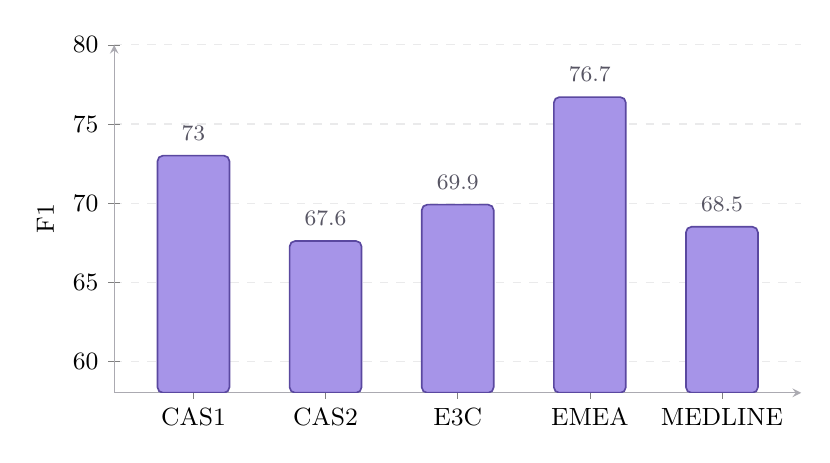
\begin{tikzpicture}
\begin{axis}[
    thesis bar,
    bar width=26pt,
    ymin=58, ymax=80,
    ylabel={F1},
    symbolic x coords={CAS1,CAS2,E3C,EMEA,MEDLINE},
    xtick=data,
    nodes near coords,
    nodes near coords align={vertical},
    nodes near coords style={font=\footnotesize, color=Ink!80, yshift=2pt},
    every node near coord/.append style={/pgf/number format/.cd, fixed, precision=1},
]
\addplot[fill=Primary, draw=PrimaryDark, line width=0.6pt, rounded corners=2pt]
    coordinates {(CAS1,73.0) (CAS2,67.6) (E3C,69.9) (EMEA,76.7) (MEDLINE,68.5)};
\end{axis}
\end{tikzpicture}
\caption{\textbf{Style A} --- Single series with value labels.}
\label{fig:bar-a}
\end{figure}

\bigskip

%% --- BAR B ---
\subsection{Style B — Two series (ours vs baseline)}

\begin{figure}[h]
\centering
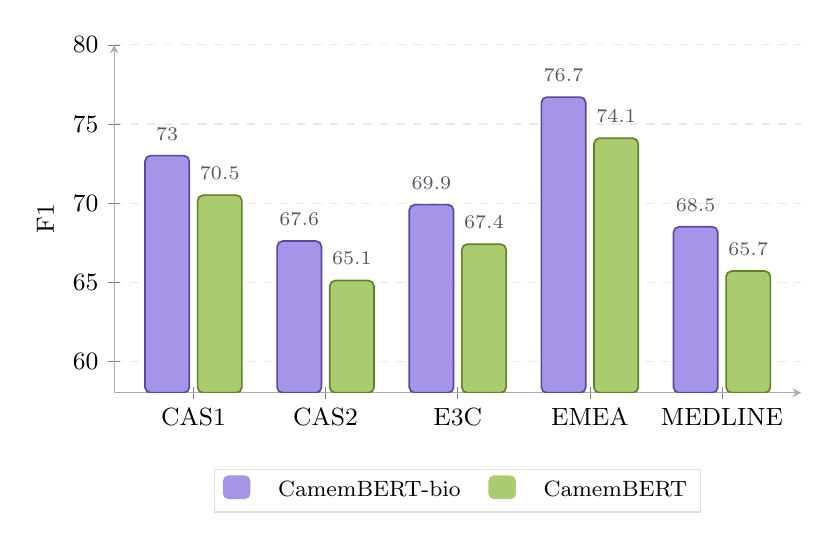
\begin{tikzpicture}
\begin{axis}[
    thesis bar,
    bar width=16pt,
    ymin=58, ymax=80,
    ylabel={F1},
    symbolic x coords={CAS1,CAS2,E3C,EMEA,MEDLINE},
    xtick=data,
    nodes near coords,
    nodes near coords align={vertical},
    nodes near coords style={font=\scriptsize, color=Ink!80, yshift=2pt},
    every node near coord/.append style={/pgf/number format/.cd, fixed, precision=1},
]
\addplot[fill=Primary, draw=PrimaryDark, line width=0.6pt, rounded corners=2pt]
    coordinates {(CAS1,73.0) (CAS2,67.6) (E3C,69.9) (EMEA,76.7) (MEDLINE,68.5)};
\addplot[fill=Secondary, draw=SecondaryDark, line width=0.6pt, rounded corners=2pt]
    coordinates {(CAS1,70.5) (CAS2,65.1) (E3C,67.4) (EMEA,74.1) (MEDLINE,65.7)};
\legend{CamemBERT-bio, CamemBERT}
\end{axis}
\end{tikzpicture}
\caption{\textbf{Style B} --- Two series with value labels and legend.}
\label{fig:bar-b}
\end{figure}

\newpage

%% --- BAR D ---
\subsection{Style D — Two series with error bars ($\pm$ std)}

\begin{figure}[h]
\centering
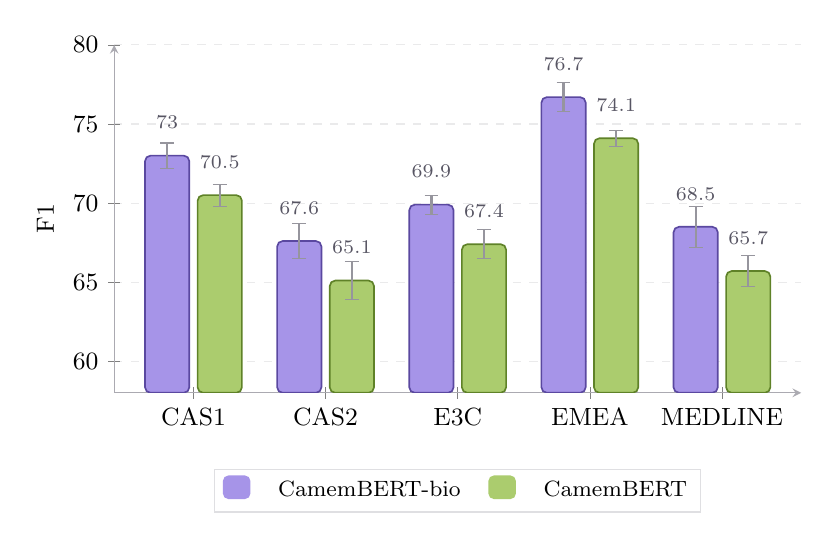
\begin{tikzpicture}
\begin{axis}[
    thesis bar,
    bar width=16pt,
    ymin=58, ymax=80,
    ylabel={F1},
    symbolic x coords={CAS1,CAS2,E3C,EMEA,MEDLINE},
    xtick=data,
    nodes near coords,
    nodes near coords align={vertical},
    nodes near coords style={font=\scriptsize, color=Ink!80, yshift=6pt},
    every node near coord/.append style={/pgf/number format/.cd, fixed, precision=1},
    error bars/y dir=both,
    error bars/y explicit,
    error bars/error bar style={line width=0.8pt, Ink!50},
    error bars/error mark options={rotate=90, Ink!50, mark size=2.5pt},
]
\addplot[fill=Primary, draw=PrimaryDark, line width=0.6pt, rounded corners=2pt]
    coordinates {
        (CAS1,73.0) +- (0,0.8)
        (CAS2,67.6) +- (0,1.1)
        (E3C,69.9)  +- (0,0.6)
        (EMEA,76.7) +- (0,0.9)
        (MEDLINE,68.5) +- (0,1.3)
    };
\addplot[fill=Secondary, draw=SecondaryDark, line width=0.6pt, rounded corners=2pt,
    error bars/y dir=both, error bars/y explicit,
    error bars/error bar style={line width=0.8pt, Ink!50},
    error bars/error mark options={rotate=90, Ink!50, mark size=2.5pt}]
    coordinates {
        (CAS1,70.5) +- (0,0.7)
        (CAS2,65.1) +- (0,1.2)
        (E3C,67.4)  +- (0,0.9)
        (EMEA,74.1) +- (0,0.5)
        (MEDLINE,65.7) +- (0,1.0)
    };
\legend{CamemBERT-bio, CamemBERT}
\end{axis}
\end{tikzpicture}
\caption{\textbf{Style D} --- Two series with error bars ($\pm$ std).}
\label{fig:bar-d}
\end{figure}

\newpage

%% ============================================================
\section{Line Plots}
\label{sec:lineplots}
%% ============================================================

Same visual language as barplots: open axes, dashed y-grid, legend below, palette-matched colors with dark borders on markers. Our model gets a thicker line (2.5pt) + confidence band; baselines are thinner (1.5pt) with distinct dash patterns. Markers have visible dark borders matching the bar chart treatment.

\bigskip

\subsection{Style A — Markers with bordered fills}

\begin{figure}[h]
\centering
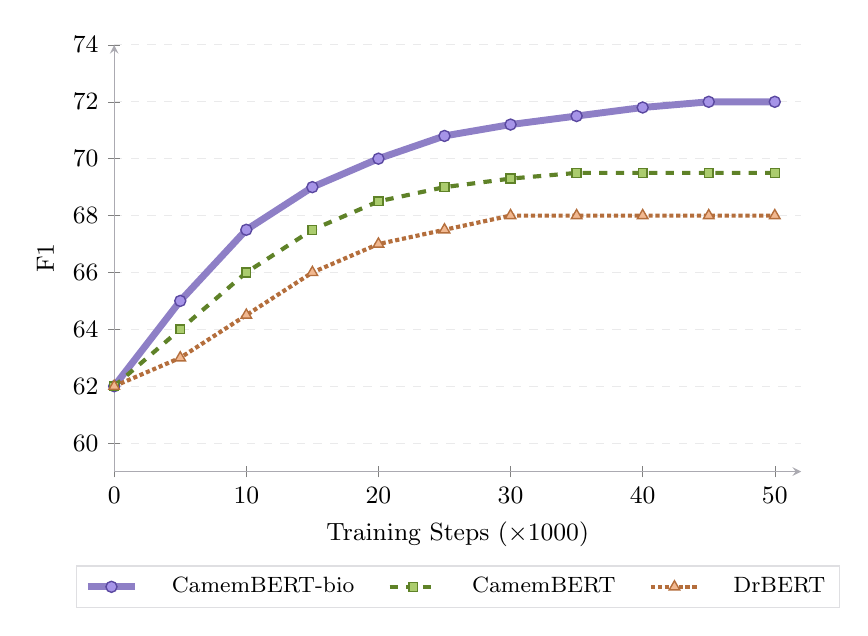
\begin{tikzpicture}
\begin{axis}[
    thesis line,
    xlabel={Training Steps ($\times$1000)},
    ylabel={F1},
    xmin=0, xmax=52,
    ymin=59, ymax=74,
    xtick={0,10,20,30,40,50},
    ytick={60,62,64,66,68,70,72,74},
]
\addplot[Primary!80!Ink, line width=2.5pt, mark=*, mark size=2pt,
    mark options={solid, fill=Primary, draw=PrimaryDark, line width=0.5pt}]
    coordinates {(0,62) (5,65) (10,67.5) (15,69) (20,70) (25,70.8) (30,71.2) (35,71.5) (40,71.8) (45,72) (50,72)};
\addplot[SecondaryDark, line width=1.5pt, dashed, mark=square*, mark size=1.6pt,
    mark options={solid, fill=Secondary, draw=SecondaryDark, line width=0.5pt}]
    coordinates {(0,62) (5,64) (10,66) (15,67.5) (20,68.5) (25,69) (30,69.3) (35,69.5) (40,69.5) (45,69.5) (50,69.5)};
\addplot[TertiaryDark, line width=1.5pt, densely dotted, mark=triangle*, mark size=2.2pt,
    mark options={solid, fill=Tertiary, draw=TertiaryDark, line width=0.5pt}]
    coordinates {(0,62) (5,63) (10,64.5) (15,66) (20,67) (25,67.5) (30,68) (35,68) (40,68) (45,68) (50,68)};
\legend{CamemBERT-bio, CamemBERT, DrBERT}
\end{axis}
\end{tikzpicture}
\caption{\textbf{Style A} --- Bordered markers matching bar chart borders. Thicker line + circle for our model; dashed/dotted + square/triangle for baselines.}
\label{fig:line-a}
\end{figure}

\bigskip

\subsection{Style B — Markers + confidence band on our model}

\begin{figure}[h]
\centering
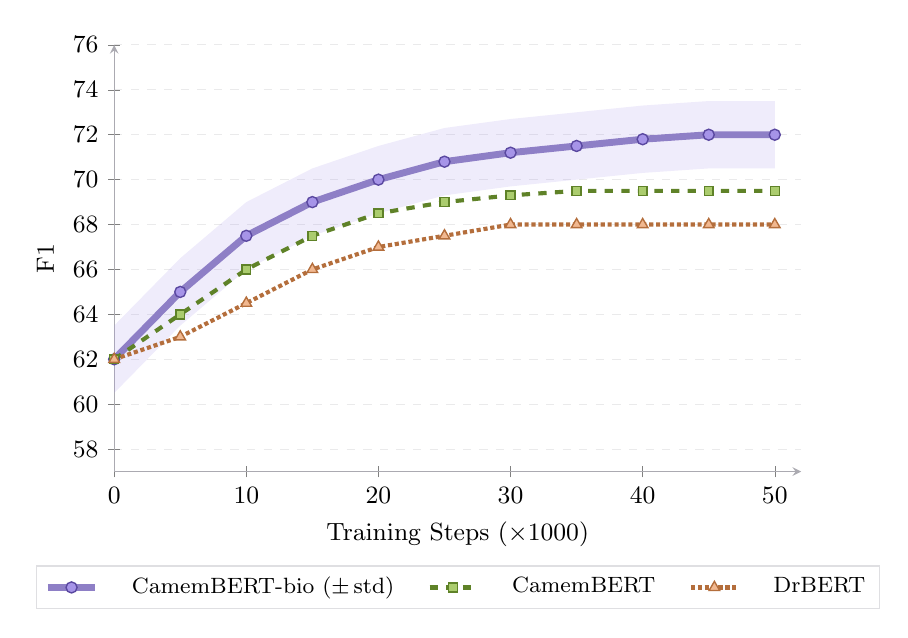
\begin{tikzpicture}
\begin{axis}[
    thesis line,
    xlabel={Training Steps ($\times$1000)},
    ylabel={F1},
    xmin=0, xmax=52,
    ymin=57, ymax=76,
    xtick={0,10,20,30,40,50},
    ytick={58,60,62,64,66,68,70,72,74,76},
]
% Confidence band for our model
\addplot[name path=upper, draw=none, forget plot]
    coordinates {(0,63.5) (5,66.5) (10,69) (15,70.5) (20,71.5) (25,72.3) (30,72.7) (35,73) (40,73.3) (45,73.5) (50,73.5)};
\addplot[name path=lower, draw=none, forget plot]
    coordinates {(0,60.5) (5,63.5) (10,66) (15,67.5) (20,68.5) (25,69.3) (30,69.7) (35,70) (40,70.3) (45,70.5) (50,70.5)};
\addplot[fill=Primary, fill opacity=0.18, forget plot, draw=none] fill between[of=upper and lower];
% Main lines with bordered markers
\addplot[Primary!80!Ink, line width=2.5pt, mark=*, mark size=2pt,
    mark options={solid, fill=Primary, draw=PrimaryDark, line width=0.5pt}]
    coordinates {(0,62) (5,65) (10,67.5) (15,69) (20,70) (25,70.8) (30,71.2) (35,71.5) (40,71.8) (45,72) (50,72)};
\addplot[SecondaryDark, line width=1.5pt, dashed, mark=square*, mark size=1.6pt,
    mark options={solid, fill=Secondary, draw=SecondaryDark, line width=0.5pt}]
    coordinates {(0,62) (5,64) (10,66) (15,67.5) (20,68.5) (25,69) (30,69.3) (35,69.5) (40,69.5) (45,69.5) (50,69.5)};
\addplot[TertiaryDark, line width=1.5pt, densely dotted, mark=triangle*, mark size=2.2pt,
    mark options={solid, fill=Tertiary, draw=TertiaryDark, line width=0.5pt}]
    coordinates {(0,62) (5,63) (10,64.5) (15,66) (20,67) (25,67.5) (30,68) (35,68) (40,68) (45,68) (50,68)};
\legend{CamemBERT-bio ($\pm$\,std), CamemBERT, DrBERT}
\end{axis}
\end{tikzpicture}
\caption{\textbf{Style B} --- Same markers as A, plus confidence band ($\pm$ std) on our model only.}
\label{fig:line-b}
\end{figure}

\newpage

%% ============================================================
\section{Pipeline / Architecture Diagrams}
\label{sec:pipelines}
%% ============================================================

Same palette: lavender for our model/result, lime for input data, peach for processing, steel gray for evaluation. Rounded corners, thin borders, metadata annotations below.

\bigskip

%% --- PIPELINE A: Horizontal ---
\subsection{Style A — Horizontal, color-coded stages}

\begin{figure}[h]
\centering
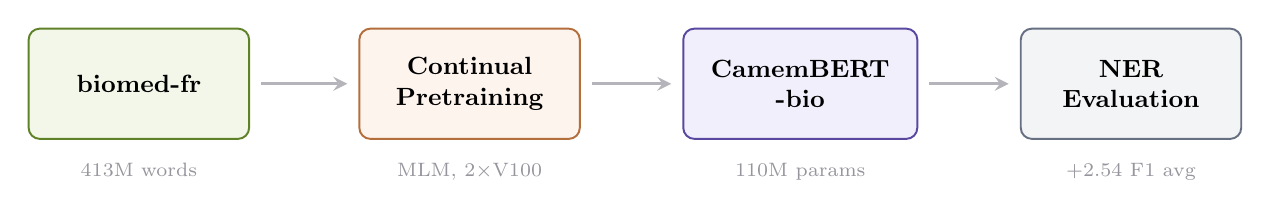
\begin{tikzpicture}[
    box/.style={rectangle, rounded corners=4pt, minimum height=1.4cm, minimum width=2.8cm,
                align=center, font=\small\bfseries, line width=0.7pt, inner xsep=10pt, inner ysep=6pt},
    arr/.style={->, line width=1.2pt, Ink!35, >=stealth, shorten >=4pt, shorten <=4pt},
]
\node[box, draw=SecondaryDark, fill=Secondary!15]
      (corpus) at (0,0) {biomed-fr};
\node[box, draw=TertiaryDark, fill=Tertiary!15]
      (pretrain) at (4.2,0) {Continual\\Pretraining};
\node[box, draw=PrimaryDark, fill=Primary!15]
      (model) at (8.4,0) {CamemBERT\\-bio};
\node[box, draw=Neutral, fill=Neutral!8]
      (eval) at (12.6,0) {NER\\Evaluation};

\draw[arr] (corpus) -- (pretrain);
\draw[arr] (pretrain) -- (model);
\draw[arr] (model) -- (eval);

\node[below=5pt, font=\scriptsize, Ink!50] at (corpus.south) {413M words};
\node[below=5pt, font=\scriptsize, Ink!50] at (pretrain.south) {MLM, 2$\times$V100};
\node[below=5pt, font=\scriptsize, Ink!50] at (model.south) {110M params};
\node[below=5pt, font=\scriptsize, Ink!50] at (eval.south) {+2.54 F1 avg};
\end{tikzpicture}
\caption{\textbf{Style A} --- Horizontal pipeline. Input (lime), process (peach), result (lavender), evaluation (gray).}
\label{fig:pipe-a}
\end{figure}

\bigskip

%% --- PIPELINE B: Vertical fork ---
\subsection{Style B — Vertical with branching}

\begin{figure}[h]
\centering
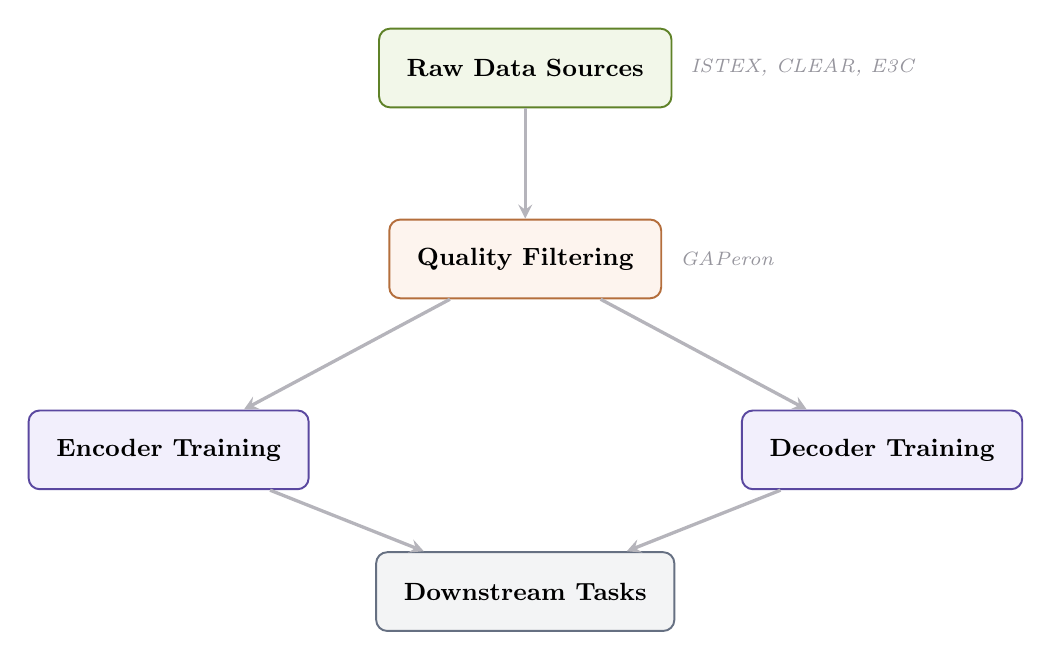
\begin{tikzpicture}[
    input/.style={rectangle, rounded corners=4pt, draw=SecondaryDark, fill=Secondary!15,
                  minimum height=1cm, minimum width=3cm, align=center, font=\small\bfseries, line width=0.7pt, inner xsep=10pt, inner ysep=6pt},
    process/.style={rectangle, rounded corners=4pt, draw=TertiaryDark, fill=Tertiary!15,
                    minimum height=1cm, minimum width=3cm, align=center, font=\small\bfseries, line width=0.7pt, inner xsep=10pt, inner ysep=6pt},
    result/.style={rectangle, rounded corners=4pt, draw=PrimaryDark, fill=Primary!15,
                   minimum height=1cm, minimum width=3cm, align=center, font=\small\bfseries, line width=0.7pt, inner xsep=10pt, inner ysep=6pt},
    eval/.style={rectangle, rounded corners=4pt, draw=Neutral, fill=Neutral!8,
                 minimum height=1cm, minimum width=3cm, align=center, font=\small\bfseries, line width=0.7pt, inner xsep=10pt, inner ysep=6pt},
    arr/.style={->, line width=1.2pt, Ink!35, >=stealth},
    node distance=1.4cm,
]
\node[input] (data) {Raw Data Sources};
\node[process, below=of data] (filter) {Quality Filtering};
\node[result, below left=1.4cm and 1cm of filter] (encoder) {Encoder Training};
\node[result, below right=1.4cm and 1cm of filter] (decoder) {Decoder Training};
\node[eval, below=3.2cm of filter] (downstream) {Downstream Tasks};

\draw[arr] (data) -- (filter);
\draw[arr] (filter) -- (encoder);
\draw[arr] (filter) -- (decoder);
\draw[arr] (encoder) -- (downstream);
\draw[arr] (decoder) -- (downstream);

\node[right=3pt, font=\scriptsize, Ink!50] at (data.east) {\textit{ISTEX, CLEAR, E3C}};
\node[right=3pt, font=\scriptsize, Ink!50] at (filter.east) {\textit{GAPeron}};
\end{tikzpicture}
\caption{\textbf{Style B} --- Vertical fork pipeline. Color-coded by role.}
\label{fig:pipe-b}
\end{figure}

\newpage

%% ============================================================
\section{Summary — Validated Choices}
%% ============================================================

\begin{itemize}[leftmargin=2cm]
\item[\textbf{Palette:}] Palette 4 --- Lavender Haze \& Lime (Section~\ref{sec:palette})
\item[\textbf{Tables:}] Style A with lavender separators (Section~\ref{sec:tables})
\item[\textbf{Bar charts:}] A (single), B (two series), D (error bars) (Section~\ref{sec:barcharts})
\item[\textbf{Line plots:}] A (markers) and B (markers + confidence band) (Section~\ref{sec:lineplots})
\item[\textbf{Pipelines:}] A (horizontal) and B (vertical fork) (Section~\ref{sec:pipelines})
\end{itemize}

\bigskip

\noindent\textbf{Design rules across all figures:}
\begin{itemize}
\item Open axes (left + bottom only), axis color \texttt{Ink!40}
\item Dashed y-grid (\texttt{Ink!10, dashed}), no x-grid
\item Legend below plot, centered, with \texttt{column sep=8pt}
\item Serif font throughout (matching thesis body)
\item Markers with visible dark borders (like bar chart border treatment)
\item Our model: thicker lines/bolder presence; baselines: thinner, dashed/dotted
\item PDF vector output only
\end{itemize}


\newpage

%% ============================================================
%%
%%   PART II — ARCHIVE (Rejected / Alternative Styles)
%%
%% ============================================================

\part*{Archive — Rejected Styles}
\addcontentsline{toc}{part}{Archive --- Rejected Styles}

\textit{Styles considered but not selected. Kept here for reference.}

\bigskip

%% ============================================================
\section{Rejected Bar Chart: Style C — Three series (no value labels)}
%% ============================================================

\begin{figure}[h]
\centering
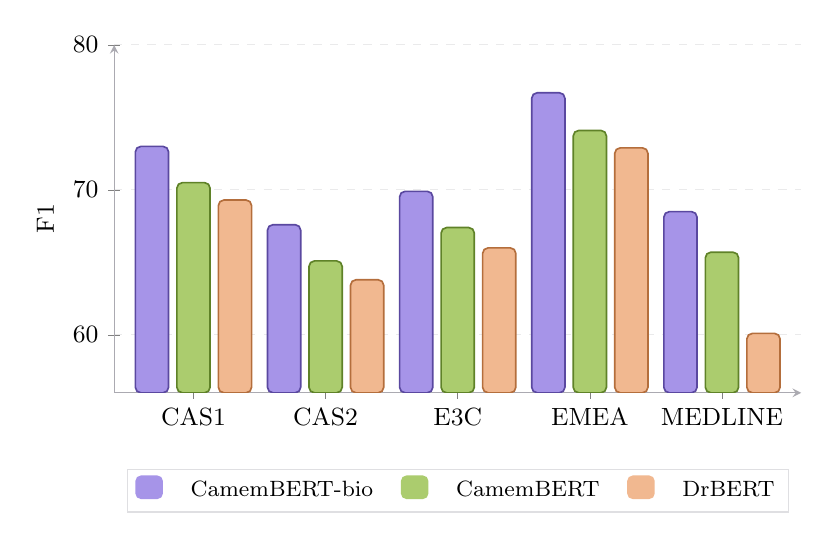
\begin{tikzpicture}
\begin{axis}[
    thesis bar,
    bar width=12pt,
    ymin=56, ymax=80,
    ylabel={F1},
    symbolic x coords={CAS1,CAS2,E3C,EMEA,MEDLINE},
    xtick=data,
]
\addplot[fill=Primary, draw=PrimaryDark, line width=0.6pt, rounded corners=2pt]
    coordinates {(CAS1,73.0) (CAS2,67.6) (E3C,69.9) (EMEA,76.7) (MEDLINE,68.5)};
\addplot[fill=Secondary, draw=SecondaryDark, line width=0.6pt, rounded corners=2pt]
    coordinates {(CAS1,70.5) (CAS2,65.1) (E3C,67.4) (EMEA,74.1) (MEDLINE,65.7)};
\addplot[fill=Tertiary, draw=TertiaryDark, line width=0.6pt, rounded corners=2pt]
    coordinates {(CAS1,69.3) (CAS2,63.8) (E3C,66.0) (EMEA,72.9) (MEDLINE,60.1)};
\legend{CamemBERT-bio, CamemBERT, DrBERT}
\end{axis}
\end{tikzpicture}
\caption{\textbf{[Rejected] Style C} --- Three series, no value labels. Too crowded for value annotations.}
\label{fig:bar-c-archive}
\end{figure}

%% ============================================================
\section{Rejected Palettes}
%% ============================================================

Alternative palettes that were not selected. Shown with mini bar + line charts.

\bigskip

%% --- Palette 1 ---
\subsection{Palette 1 — Matcha Pop \& Coral Punch}

\definecolor{P1a}{RGB}{102, 183, 141}
\definecolor{P1b}{RGB}{232, 132, 132}
\definecolor{P1c}{RGB}{241, 202, 124}
\definecolor{P1d}{RGB}{106, 118, 136}
\definecolor{P1bg}{RGB}{252, 250, 246}
\definecolor{P1text}{RGB}{38, 42, 50}

\begin{tikzpicture}
\fill[P1a] (0,0) rectangle (2.2,1.2); \node[font=\small, white] at (1.1,0.6) {Matcha};
\fill[P1b] (2.5,0) rectangle (4.7,1.2); \node[font=\small, white] at (3.6,0.6) {Coral};
\fill[P1c] (5.0,0) rectangle (7.2,1.2); \node[font=\small, P1text] at (6.1,0.6) {Citrus};
\fill[P1d] (7.5,0) rectangle (9.7,1.2); \node[font=\small, white] at (8.6,0.6) {Slate};
\fill[P1bg] (10.0,0) rectangle (12.2,1.2); \node[font=\small, P1text] at (11.1,0.6) {Paper};
\fill[P1text] (12.5,0) rectangle (14.7,1.2); \node[font=\small, white] at (13.6,0.6) {Ink};
\end{tikzpicture}

\begin{minipage}[t]{0.48\textwidth}
\centering
\begin{tikzpicture}
\begin{axis}[
    ybar=3pt, width=6.5cm, height=4.5cm, bar width=11pt,
    ymin=60, ymax=80, ylabel={F1}, ylabel style={font=\small},
    symbolic x coords={CAS1,CAS2,E3C,EMEA}, xtick=data,
    tick label style={font=\small}, ytick={60,65,70,75},
    axis line style={P1text}, grid=none, enlarge x limits=0.25,
    legend style={at={(0.98,0.98)}, anchor=north east, font=\scriptsize, draw=P1d, fill=P1bg},
]
\addplot[fill=P1a, draw=P1text!60, line width=0.6pt] coordinates {(CAS1,73.0) (CAS2,67.6) (E3C,69.9) (EMEA,76.7)};
\addplot[fill=P1b, draw=P1text!60, line width=0.6pt] coordinates {(CAS1,70.5) (CAS2,65.1) (E3C,67.4) (EMEA,74.1)};
\legend{Ours, Baseline}
\end{axis}
\end{tikzpicture}
\end{minipage}%
\hfill
\begin{minipage}[t]{0.48\textwidth}
\centering
\begin{tikzpicture}
\begin{axis}[
    width=6.5cm, height=4.5cm, grid=none,
    xmin=0, xmax=50, ymin=60, ymax=75,
    tick label style={font=\small}, axis line style={P1text},
    ylabel={F1}, ylabel style={font=\small},
    legend style={at={(0.98,0.02)}, anchor=south east, font=\scriptsize, draw=P1d, fill=P1bg},
]
\addplot[P1a, line width=2pt, mark=square*, mark size=2pt, mark options={fill=P1a}] coordinates {(0,62) (10,67.5) (20,70) (30,71.2) (40,71.8) (50,72)};
\addplot[P1b, line width=1.5pt, dashed, mark=triangle*, mark size=2.5pt, mark options={fill=P1b}] coordinates {(0,62) (10,66) (20,68.5) (30,69.3) (40,69.5) (50,69.5)};
\addplot[P1c, line width=1.5pt, dotted, mark=diamond*, mark size=2.5pt, mark options={fill=P1c}] coordinates {(0,62) (10,64.5) (20,67) (30,68) (40,68) (50,68)};
\legend{CB-bio, CamemBERT, DrBERT}
\end{axis}
\end{tikzpicture}
\end{minipage}

\bigskip\bigskip

%% --- Palette 2 ---
\subsection{Palette 2 — Skyline Blue \& Tangerine}

\definecolor{P2a}{RGB}{86, 134, 224}
\definecolor{P2b}{RGB}{236, 157, 101}
\definecolor{P2c}{RGB}{141, 165, 229}
\definecolor{P2d}{RGB}{125, 136, 148}
\definecolor{P2bg}{RGB}{250, 248, 244}
\definecolor{P2text}{RGB}{34, 38, 47}

\begin{tikzpicture}
\fill[P2a] (0,0) rectangle (2.2,1.2); \node[font=\small, white] at (1.1,0.6) {Skyline};
\fill[P2b] (2.5,0) rectangle (4.7,1.2); \node[font=\small, P2text] at (3.6,0.6) {Tangerine};
\fill[P2c] (5.0,0) rectangle (7.2,1.2); \node[font=\small, white] at (6.1,0.6) {Cobalt};
\fill[P2d] (7.5,0) rectangle (9.7,1.2); \node[font=\small, white] at (8.6,0.6) {Sage};
\fill[P2bg] (10.0,0) rectangle (12.2,1.2); \node[font=\small, P2text] at (11.1,0.6) {Paper};
\fill[P2text] (12.5,0) rectangle (14.7,1.2); \node[font=\small, white] at (13.6,0.6) {Ink};
\end{tikzpicture}

\begin{minipage}[t]{0.48\textwidth}
\centering
\begin{tikzpicture}
\begin{axis}[
    ybar=3pt, width=6.5cm, height=4.5cm, bar width=11pt,
    ymin=60, ymax=80, ylabel={F1}, ylabel style={font=\small},
    symbolic x coords={CAS1,CAS2,E3C,EMEA}, xtick=data,
    tick label style={font=\small}, ytick={60,65,70,75},
    axis line style={P2text}, grid=none, enlarge x limits=0.25,
    legend style={at={(0.98,0.98)}, anchor=north east, font=\scriptsize, draw=P2d, fill=P2bg},
]
\addplot[fill=P2a, draw=P2text!60, line width=0.6pt] coordinates {(CAS1,73.0) (CAS2,67.6) (E3C,69.9) (EMEA,76.7)};
\addplot[fill=P2b, draw=P2text!60, line width=0.6pt] coordinates {(CAS1,70.5) (CAS2,65.1) (E3C,67.4) (EMEA,74.1)};
\legend{Ours, Baseline}
\end{axis}
\end{tikzpicture}
\end{minipage}%
\hfill
\begin{minipage}[t]{0.48\textwidth}
\centering
\begin{tikzpicture}
\begin{axis}[
    width=6.5cm, height=4.5cm, grid=none,
    xmin=0, xmax=50, ymin=60, ymax=75,
    tick label style={font=\small}, axis line style={P2text},
    ylabel={F1}, ylabel style={font=\small},
    legend style={at={(0.98,0.02)}, anchor=south east, font=\scriptsize, draw=P2d, fill=P2bg},
]
\addplot[P2a, line width=2pt, mark=square*, mark size=2pt, mark options={fill=P2a}] coordinates {(0,62) (10,67.5) (20,70) (30,71.2) (40,71.8) (50,72)};
\addplot[P2b, line width=1.5pt, dashed, mark=triangle*, mark size=2.5pt, mark options={fill=P2b}] coordinates {(0,62) (10,66) (20,68.5) (30,69.3) (40,69.5) (50,69.5)};
\addplot[P2c, line width=1.5pt, dotted, mark=diamond*, mark size=2.5pt, mark options={fill=P2c}] coordinates {(0,62) (10,64.5) (20,67) (30,68) (40,68) (50,68)};
\legend{CB-bio, CamemBERT, DrBERT}
\end{axis}
\end{tikzpicture}
\end{minipage}

\bigskip\bigskip

%% --- Palette 3 ---
\subsection{Palette 3 — Bubblegum \& Graphite}

\definecolor{P3a}{RGB}{205, 105, 157}
\definecolor{P3b}{RGB}{68, 74, 88}
\definecolor{P3c}{RGB}{152, 160, 174}
\definecolor{P3d}{RGB}{224, 227, 233}
\definecolor{P3bg}{RGB}{252, 251, 248}
\definecolor{P3text}{RGB}{40, 41, 46}

\begin{tikzpicture}
\fill[P3a] (0,0) rectangle (2.2,1.2); \node[font=\small, white] at (1.1,0.6) {Bubblegum};
\fill[P3b] (2.5,0) rectangle (4.7,1.2); \node[font=\small, white] at (3.6,0.6) {Graphite};
\fill[P3c] (5.0,0) rectangle (7.2,1.2); \node[font=\small, white] at (6.1,0.6) {Cloud};
\fill[P3d] (7.5,0) rectangle (9.7,1.2); \node[font=\small, P3text] at (8.6,0.6) {Light};
\fill[P3bg] (10.0,0) rectangle (12.2,1.2); \node[font=\small, P3text] at (11.1,0.6) {Paper};
\fill[P3text] (12.5,0) rectangle (14.7,1.2); \node[font=\small, white] at (13.6,0.6) {Ink};
\end{tikzpicture}

\begin{minipage}[t]{0.48\textwidth}
\centering
\begin{tikzpicture}
\begin{axis}[
    ybar=3pt, width=6.5cm, height=4.5cm, bar width=11pt,
    ymin=60, ymax=80, ylabel={F1}, ylabel style={font=\small},
    symbolic x coords={CAS1,CAS2,E3C,EMEA}, xtick=data,
    tick label style={font=\small}, ytick={60,65,70,75},
    axis line style={P3text}, grid=none, enlarge x limits=0.25,
    legend style={at={(0.98,0.98)}, anchor=north east, font=\scriptsize, draw=P3c, fill=P3bg},
]
\addplot[fill=P3a, draw=P3text!60, line width=0.6pt] coordinates {(CAS1,73.0) (CAS2,67.6) (E3C,69.9) (EMEA,76.7)};
\addplot[fill=P3b, draw=P3text!60, line width=0.6pt] coordinates {(CAS1,70.5) (CAS2,65.1) (E3C,67.4) (EMEA,74.1)};
\legend{Ours, Baseline}
\end{axis}
\end{tikzpicture}
\end{minipage}%
\hfill
\begin{minipage}[t]{0.48\textwidth}
\centering
\begin{tikzpicture}
\begin{axis}[
    width=6.5cm, height=4.5cm, grid=none,
    xmin=0, xmax=50, ymin=60, ymax=75,
    tick label style={font=\small}, axis line style={P3text},
    ylabel={F1}, ylabel style={font=\small},
    legend style={at={(0.98,0.02)}, anchor=south east, font=\scriptsize, draw=P3c, fill=P3bg},
]
\addplot[P3a, line width=2.5pt, mark=square*, mark size=2pt, mark options={fill=P3a}] coordinates {(0,62) (10,67.5) (20,70) (30,71.2) (40,71.8) (50,72)};
\addplot[P3b, line width=1.5pt, dashed, mark=triangle*, mark size=2.5pt, mark options={fill=P3b}] coordinates {(0,62) (10,66) (20,68.5) (30,69.3) (40,69.5) (50,69.5)};
\addplot[P3c, line width=1.5pt, dotted, mark=diamond*, mark size=2pt, mark options={fill=P3c}] coordinates {(0,62) (10,64.5) (20,67) (30,68) (40,68) (50,68)};
\legend{CB-bio, CamemBERT, DrBERT}
\end{axis}
\end{tikzpicture}
\end{minipage}

\bigskip\bigskip

%% --- Palette 5 ---
\subsection{Palette 5 — Aqua Neon \& Cherry}

\definecolor{P5a}{RGB}{66, 170, 178}
\definecolor{P5b}{RGB}{198, 95, 115}
\definecolor{P5c}{RGB}{238, 176, 96}
\definecolor{P5d}{RGB}{122, 134, 144}
\definecolor{P5bg}{RGB}{247, 250, 251}
\definecolor{P5text}{RGB}{34, 43, 49}

\begin{tikzpicture}
\fill[P5a] (0,0) rectangle (2.2,1.2); \node[font=\small, white] at (1.1,0.6) {Aqua};
\fill[P5b] (2.5,0) rectangle (4.7,1.2); \node[font=\small, white] at (3.6,0.6) {Cherry};
\fill[P5c] (5.0,0) rectangle (7.2,1.2); \node[font=\small, P5text] at (6.1,0.6) {Mango};
\fill[P5d] (7.5,0) rectangle (9.7,1.2); \node[font=\small, white] at (8.6,0.6) {Slate};
\fill[P5bg] (10.0,0) rectangle (12.2,1.2); \node[font=\small, P5text] at (11.1,0.6) {Paper};
\fill[P5text] (12.5,0) rectangle (14.7,1.2); \node[font=\small, white] at (13.6,0.6) {Ink};
\end{tikzpicture}

\begin{minipage}[t]{0.48\textwidth}
\centering
\begin{tikzpicture}
\begin{axis}[
    ybar=3pt, width=6.5cm, height=4.5cm, bar width=11pt,
    ymin=60, ymax=80, ylabel={F1}, ylabel style={font=\small},
    symbolic x coords={CAS1,CAS2,E3C,EMEA}, xtick=data,
    tick label style={font=\small}, ytick={60,65,70,75},
    axis line style={P5text}, grid=none, enlarge x limits=0.25,
    legend style={at={(0.98,0.98)}, anchor=north east, font=\scriptsize, draw=P5d, fill=P5bg},
]
\addplot[fill=P5a, draw=P5text!60, line width=0.6pt] coordinates {(CAS1,73.0) (CAS2,67.6) (E3C,69.9) (EMEA,76.7)};
\addplot[fill=P5b, draw=P5text!60, line width=0.6pt] coordinates {(CAS1,70.5) (CAS2,65.1) (E3C,67.4) (EMEA,74.1)};
\legend{Ours, Baseline}
\end{axis}
\end{tikzpicture}
\end{minipage}%
\hfill
\begin{minipage}[t]{0.48\textwidth}
\centering
\begin{tikzpicture}
\begin{axis}[
    width=6.5cm, height=4.5cm, grid=none,
    xmin=0, xmax=50, ymin=60, ymax=75,
    tick label style={font=\small}, axis line style={P5text},
    ylabel={F1}, ylabel style={font=\small},
    legend style={at={(0.98,0.02)}, anchor=south east, font=\scriptsize, draw=P5d, fill=P5bg},
]
\addplot[P5a, line width=2pt, mark=square*, mark size=2pt, mark options={fill=P5a}] coordinates {(0,62) (10,67.5) (20,70) (30,71.2) (40,71.8) (50,72)};
\addplot[P5b, line width=1.5pt, dashed, mark=triangle*, mark size=2.5pt, mark options={fill=P5b}] coordinates {(0,62) (10,66) (20,68.5) (30,69.3) (40,69.5) (50,69.5)};
\addplot[P5c, line width=1.5pt, dotted, mark=diamond*, mark size=2.5pt, mark options={fill=P5c}] coordinates {(0,62) (10,64.5) (20,67) (30,68) (40,68) (50,68)};
\legend{CB-bio, CamemBERT, DrBERT}
\end{axis}
\end{tikzpicture}
\end{minipage}

\bigskip\bigskip

%% --- Palette 6 ---
\subsection{Palette 6 — Electric Mint \& Mocha Chrome}

\definecolor{P6a}{RGB}{100, 182, 160}
\definecolor{P6b}{RGB}{88, 79, 98}
\definecolor{P6c}{RGB}{169, 161, 178}
\definecolor{P6d}{RGB}{224, 220, 228}
\definecolor{P6bg}{RGB}{250, 248, 246}
\definecolor{P6text}{RGB}{44, 40, 50}

\begin{tikzpicture}
\fill[P6a] (0,0) rectangle (2.2,1.2); \node[font=\small, white] at (1.1,0.6) {Mint};
\fill[P6b] (2.5,0) rectangle (4.7,1.2); \node[font=\small, white] at (3.6,0.6) {Mocha};
\fill[P6c] (5.0,0) rectangle (7.2,1.2); \node[font=\small, white] at (6.1,0.6) {Lilac gray};
\fill[P6d] (7.5,0) rectangle (9.7,1.2); \node[font=\small, P6text] at (8.6,0.6) {Light};
\fill[P6bg] (10.0,0) rectangle (12.2,1.2); \node[font=\small, P6text] at (11.1,0.6) {Cream};
\fill[P6text] (12.5,0) rectangle (14.7,1.2); \node[font=\small, white] at (13.6,0.6) {Ink};
\end{tikzpicture}

\begin{minipage}[t]{0.48\textwidth}
\centering
\begin{tikzpicture}
\begin{axis}[
    ybar=3pt, width=6.5cm, height=4.5cm, bar width=11pt,
    ymin=60, ymax=80, ylabel={F1}, ylabel style={font=\small},
    symbolic x coords={CAS1,CAS2,E3C,EMEA}, xtick=data,
    tick label style={font=\small}, ytick={60,65,70,75},
    axis line style={P6text}, grid=none, enlarge x limits=0.25,
    legend style={at={(0.98,0.98)}, anchor=north east, font=\scriptsize, draw=P6c, fill=P6bg},
]
\addplot[fill=P6a, draw=P6text!60, line width=0.6pt] coordinates {(CAS1,73.0) (CAS2,67.6) (E3C,69.9) (EMEA,76.7)};
\addplot[fill=P6b, draw=P6text!60, line width=0.6pt] coordinates {(CAS1,70.5) (CAS2,65.1) (E3C,67.4) (EMEA,74.1)};
\legend{Ours, Baseline}
\end{axis}
\end{tikzpicture}
\end{minipage}%
\hfill
\begin{minipage}[t]{0.48\textwidth}
\centering
\begin{tikzpicture}
\begin{axis}[
    width=6.5cm, height=4.5cm, grid=none,
    xmin=0, xmax=50, ymin=60, ymax=75,
    tick label style={font=\small}, axis line style={P6text},
    ylabel={F1}, ylabel style={font=\small},
    legend style={at={(0.98,0.02)}, anchor=south east, font=\scriptsize, draw=P6c, fill=P6bg},
]
\addplot[P6a, line width=2.5pt, mark=square*, mark size=2pt, mark options={fill=P6a}] coordinates {(0,62) (10,67.5) (20,70) (30,71.2) (40,71.8) (50,72)};
\addplot[P6b, line width=1.5pt, dashed, mark=triangle*, mark size=2.5pt, mark options={fill=P6b}] coordinates {(0,62) (10,66) (20,68.5) (30,69.3) (40,69.5) (50,69.5)};
\addplot[P6c, line width=1.5pt, dotted, mark=diamond*, mark size=2pt, mark options={fill=P6c}] coordinates {(0,62) (10,64.5) (20,67) (30,68) (40,68) (50,68)};
\legend{CB-bio, CamemBERT, DrBERT}
\end{axis}
\end{tikzpicture}
\end{minipage}

\end{document}
